\section{Experiments and Results}\label{sec:experimentsandresults}
We conducted experiments using ICLab and RIPE Atlas. ICLab is a research platform used to measure global Internet censorship. ICLab was used to conduct tests targeted at over 800 domains. The domains tested fall in a variety of categories, including the  top 500 Alexa domains as accessed by people within Iran as well as several hundred additional domains, which were previously reported to be blocked. RIPE Atlas is a global network of probes that measure Internet reachability and connectivity.  RIPE was used determine several vantage points from which to send DNS queries. 

\subsection{ICLab}
ICLab platform was used to conduct DNS, traceroute, TCP connect, TLS handshake and HTTP GET measurements. All except the traceroute experiments were successful.
\subsubsection{DNS} DNS resolution of each domain in our list was conducted from the Iranian VP using two resolvers: A local resolver of the VP's choice and the google resolver, 8.8.8.8 were used. A python script was then used to compare the DNS responses from a US-based VP to the results obtained from Iran.\\ 
All queries using the google resolver yielded a null response. We hypothesize the DNS packets destined to 8.8.8.8 are dropped. Some queries using the local resolver also yielded a null response even though a valid IP was obtained for the query using the US-based VP. On the flip side, a few domains in our test list got null response in the US and a valid IP in Iran. Figure \reminder x shows a comparison of DNS responses from a US VP and a Iranian VP.\\

\begin{figure}
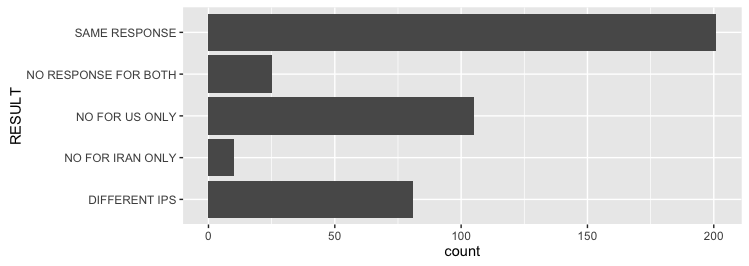
\includegraphics[
  height=.5\columnwidth,
  width=.9\columnwidth
]{pictures/DNSComparision.png}
  \caption{This is a teaser}
  \label{fig:DNSCompare}
\end{figure}

\subsubsection{Traceroute} We setup our experiment to conduct traceroute measurements before we handed it over to the person responsible for ICLab. Our intention was to pinpoint the location of the censor within Iran’s network by using the traceroute emasurements. However, we got "traceroute not found or not installed" error for all of our measurements. We see this as one of the limitations of the ICLab platform compared to RIPE atlas. Researchers do not control the remote machines in the test countries so they lack a clear expectations of what kinds of tests will be successful. \\
\subsubsection{TCP connect} 
\subsubsection{TLS handshake}
\subsubsection{HTTP}
 HTTP GET requests were executed from VPs  in both the United States and Iran to use as control and experiment results, respectively. The same test list of more than 500 urls was used. ICLab separates an url into host and path using a python library, \textit{urllib}. HTTP GET requests to invalid domains were used to verify Deep Packet Inspection(DPI). For this, paths to Alexa top websites in Iran were modified with a trigger word such as porn. The expectation is that an invalid domain should return a 404 Page Not Found Error.\\
HTTP GET requests gave a more representative view of censorship in Iran. Many domains with successful TCP handshake gave 4xx responses. We believe that  the TCP connect succeeds because the collateral damage of IP-based blocking has deterred Iran from conducting IP-based blocking. While mix of status codes 200, 400, 3xx, 403 and 404 were obtained from the Iranian VP, the same test list of URLs resulted in a negligible number of failures when run from a U.S-based VP.  A handful of error responses gotten for the US VP were usually  404 Page Not Found or 403 Forbidden. 404 error occurred in the case where the domain name was intentionally invalid like in the case of path modification to check for deep packet inspection. Some websites such as http://ladysun.net -a Women's rights website, http://www.alrased.net/site- a minority faith website, http://www.jawanan.org and http://www.jebhemelli.org- two political reform websites and a few other websites elicited a 403 response even from the US based VP. A traceroure measurement and geoIP lookup located the destination servers to be in countries such as  Japan and the U.S.  The reason for this censorship is unknown to us and would be a good thing to look at in future studies.\\
We were also able to verify the use of DPI by iran. An invalid domain should return a 404 Page Not Found Error, however, the invalid domains which had a trigger word in the path resulted in 403 Forbidden. Adding /porn to a path always resulted in a 403 Forbidden response from Iranian VP and 404 Not Found response from a U.S-based VP. \\ 




\subsection{RIPE Atlas }

\subsubsection{DNS:}As reported in the previous study, the method used to conduct DNS hijacking is false resolutions. We encountered several domains for which the DNS resolutions returned a false redirect address, 10.10.34.36 instead of the domain’s correct IP address. \\
RIPE Atlas allowed us to set specific parameters for the DNS requests. First, we used a total of three different source probes from which our DNS requests were sent. Parties affiliated with RIPE Atlas operate the probes. Second, we specified the IP addresses of specific resolvers in a variety of locations within Iran. The constraints, from which we narrowed down our choice in resolvers by, include reliability and location. In total, the experiments used a series of three different probes and five DNS resolvers. \\
Our aim was to determine if the false resolution results vary depending on probe and/or DNS resolver. We used the top 40 most often accessed domains in Iran from Alexa as well as 20 additional domains previously reported to be victims of DNS hijacking.\\
	Our results revealed that there probe IP from which the DNS query was sent from had no effect on the accuracy of the result from any one resolver. That is to say, given two separate probes, resolving the same domain name at the same resolver, always received the same response. This suggests that all of the DNS requests were sent as is, and never tampered with on the way to the intended resolver. On the other hand, we determined that the resolver themselves were not centralized in terms of where they retrieved their rules from. In other words, the different resolvers could be inconsistent as we saw several cases of some resolvers returning false resolutions for the same domains that other resolvers returned accurate IP addresses for. As a result of this inconsistency, we compiled three categories in which our tested domains fall in.\\

\textbf{Always Resolves:} The domain names in this category were all accurately resolved. The resolutions were verified by through the use of scripts that ran the whois command to confirm the organization name matched the intended domain’s organization name. The initial tests executed 60 domain name resolution requests from three probes to three targeted resolvers. Thus each domain was tested from three probes, targeted at three solvers, for a total of 9 resolutions per domain. A domain was assigned to this category if all of the resolutions were accurate.

\textbf{ Resolves:} Our initial test of 60 domain names over three probes and three target resolvers revealed inconsistencies in resolutions. Specifically, of our first three resolvers, located in Tehran (2) and Isfahan, the results revealed that one resolver in Tehran, would consistently return accurate resolutions for domains which returned the 10.10.34.36 redirect pages by the other two resolvers. To determine whether or not this anomalous resolver was one of a kind, or if there exists true diversity in replies, depending on the chosen DNS resolver, we extended further testing. Our additional tests utilized the same three probes, with two additional resolvers in Tabriz and Zehadan. We tested every domain that returned the false redirect address in the previous round of resolutions, against these additional resolvers. We found further inconsistencies. The domain names in this category were accurately resolved by some resolvers and falsely resolved by others. This category contained a wide variety of domains in topics including: human rights, local blogs, national news and censorship circumvention.

\textbf{ Resolves:} The domain names in this category were never accurately resolved. This applies to all five resolvers. The category contained domains from topics including: political reform, gay+lesbian, international news, and western social media. The result returned from each DNS request in this category, was either no result at all, as a result of a timeout, or the redirect IP, 10.10.34.36.

Figure 1. Shows the accurate DNS resolution rate of a few of the queried domains


Figure 2. Shows the percentage accuracy per DNS resolver, of the domains that were blocked by at least one resolver (Percentage blocking per resolver location of “Bad” Domain Names).